\subsection{Need for an integrated modeling pipeline}

\todoPaul{I threw in this material for your intro section -- feel free to keep or discard as you see fit. -Geoff}

This research is designed to significantly expand and improve the capabilities of existing land use and transport models. The focus is on long-term (e.g. 30 yr) integrated planning of transportation and land use to predict the transportation related energy impacts of alternative transportation and land use plans. Currently, UrbanSim  is used by a large number of Metropolitan Planning Organizations (MPOs) to model the interactions of transportation and land use policies for the purpose of evaluating alternatives analysis for regional transportation planning. It is typically coupled to an existing MPO transportation model system, eg. a four step model.  

There are three major impediments to implementing a rigorous analysis of the effects of land use and transportation plans over multiple decades that this project will seek to overcome.

First, the lack of behavioral integration of land use and transport models means that models are loosely coupled.  As a consequence, they cannot accommodate  recent research on the interactions of travel behavior and long-term household choices, such as residence and workplace choice and vehicle ownership.  This results in nonsensical model specifications such as travel models that predict which job a worker will go to each morning, or how many vehicles a household owns - as though these were choices made every morning over breakfast.  The alternative is to model longer-term choices in the land use model and set these choices as exogenous constraints on the daily activity and travel behavior of households.  Furthermore, this loose coupling prevents the models from directly sharing information on the individual persons and households they are simulating. This leads to significant inconsistencies between the land use and transportation models.  We will enable behavioral integration across land use and transport models  that can share data in a more realistic way.

Second, many transport models use coarse representations of the transportation network. Examples include: ignoring local streets and non-motorized infrastructure, using large zones to reflect locations, ignoring non-motorized access scales. This heavily biases the models towards the automobile mode.  Our research will improve transport and land use models to represent local streets, transit service, and urban design characteristics, in order to reduce the bias towards automobile modes.

Third and finally, transportation models are advancing in behavioral realism, but computational performance has suffered. Many of the most advanced transport models are computationally limited – taking excessive time to run. This renders them useless for integration with land use models that evaluate long-term policy bundles and combine land use policies and transportation infrastructure for thirty year planning horizons. 
In this project, we seek to improve the computational performance of the integrated models by an order of magnitude or more, in order to support experimental analysis of alternative policy combinations and analysis of uncertainty.


\subsection{Background and summary of individual tools}

\subsection{Overview summary of pipeline architecture (loosest coupling)}

\begin{figure}[htb]
\center
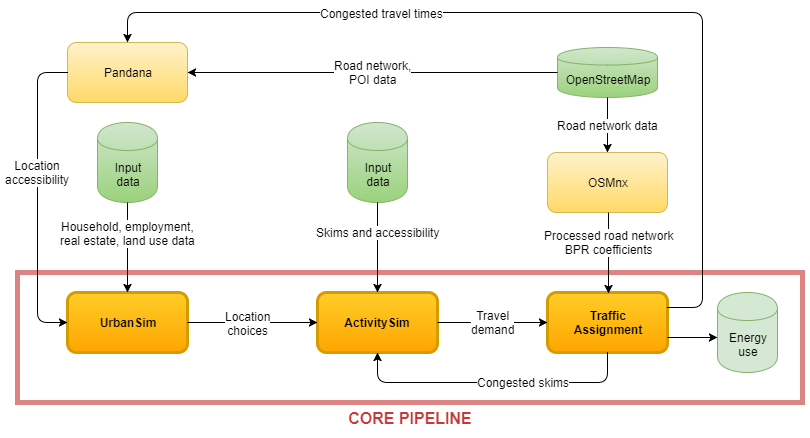
\includegraphics[width=6.5in]
{graphics/diagram_pipeline.png}
\caption{DRAFT Overview of the Integrated Modeling Pipeline's Architecture}
\label{fig:overview_pipeline_architecture}
\end{figure}




